\title{Android -- Eine Einführung}
\subtitle{Tasks \& Threads}
\author[A. Wilhelm]{Andreas Wilhelm}
\institute[www.avedo.net]{}
\titlegraphic{}
%\date{\today}
\date{CSC Computer-Schulung \& Consulting GmbH}

\begin{frame}[plain]
  \titlepage
\end{frame}

\part{Tasks \& Threads}

\section{Nebenläufigkeit unter Android}
\begin{frame}
   \frametitle{Überblick}
   \begin{itemize}
      \item Applikation läuft in einem einzigen Thread (Main- oder UI-Thread)
      \item Main-Thread verarbeitet Events und verwaltet Benutzeroberfläche
      \item Größere Operationen im Main-Thread blockieren diesen
      \item Falls Main-Thread länger als fünf Sekunden blockiert zeigt Android 
      	ANR-Dialog (Application Not Responding)
      \item Android Grafik-Toolkit eintrittsinvariant\\
      	$\rightarrow$ Komponente kann nicht aus verschiedenen Threads verwendet werden\\
      	$\rightarrow$ Änderungen an der grafischen Oberfläche nur im Main-Thread
   \end{itemize}
   
   Zwei Regeln sind im Zusammenhang mit Threads wichtig:
   \begin{enumerate}
		\item Länger andauernde Operationen sollten in Threads ausgelagert werden.
		\item Änderungen an der grafischen Oberfläche sollte nur der Main-Thread vornehmen.
	\end{enumerate}
\end{frame}

\begin{frame}
   \frametitle{Klassen}
   \begin{itemize}
      \item Android verbindet Java-Concurrent-API (\emph{java.util.concurrent}) 
      	mit Eigenimplementationen (\emph{android.os}) 
		\item Einfache Konstrukte für Nebenläufigkeit \emph{Threads} und \emph{AsyncTasks}
		\item Kommunikation mit Main-Thread über \emph{Handler}
		\item Zeitlich festgelegte oder periodische Ausführung mit 
			\emph{Timer} und \emph{ScheduledThreadPoolExecutor}
   \end{itemize}
\end{frame}

\section{Threads}
\begin{frame}
   \frametitle{Überblick}
   \begin{itemize}
      \item Verwendung von Java Threads (\emph{java.lang.Thread})
      \item Zwei Möglichkeiten Threads zu nutzen:
      	\begin{enumerate}
      		\item Ableiten von Thread und Überschreiben der \emph{run()} Methode
      		\item Übergabe eines \emph{Runnables} beim Erstellen 
      	\end{enumerate}
      \item Problem: Aktualisieren der grafischen Oberfläche:
      	\begin{enumerate}
      		\item \emph{Activity.runOnUiThread(Runnable)} führt Runnable 
      			im Main-Thread aus
      		\item Methoden \emph{post(Runnable)} und \emph{postDelayed(Runnable, long)} 
					delegieren Operation direkt an betreffendes View
      		\item Verwendung eines Handlers
      	\end{enumerate}
   \end{itemize}
\end{frame}

\begin{frame}
   \frametitle{Implementierung}
	\lstinputlisting[
		caption=Download im Thread,
		label={lst:downloadOneImage.java}]{src/java/downloadOneImage.java}
\end{frame}

\section{Handler}
\begin{frame}
   \frametitle{Probleme mit Threads}
   \begin{itemize}
     	\item Applikationen laufen in einem Thread
     	\item Blockierter Main-Thread führt zu Anzeige von ANR-Dialog
      \item Android Grafik-Toolkit eintrittsinvariant
      \item Kommunikation zwischen dem betreffenden Thread und dem Main-Thread 
      	nötig
   \end{itemize}
\end{frame}

\begin{frame}
   \frametitle{Überblick}
   \begin{itemize}
     	\item Handler ermöglicht Kommunikation mit anderen Threads
     	\item Handler wird mit genau einem Thread und dessen Nachrichten-Stapel 
			assoziiert
		\item Handler wird an erstellenden Thread gebunden
		\item Liefert Nachrichten und Operationen (\emph{Runnables}) 
			an dessen Stapel
		\item Beeinflussung der Zeitablaufsteuerung mit \emph{post*()} und \emph{send*()} 
			Methoden
		\item \emph{post*()} reihen \emph{Runnables} in den Stapel ein
		\item \emph{send*()} Methoden fügen Nachrichten dem Stapel hinzu, 
			die beim verlassen des Stapels in \emph{handleMessage()} verarbeitet werden
     	\item Handler erlauben zeitlich gebundene oder periodische 
     		Ausführung
   \end{itemize}
\end{frame}

\begin{frame}
   \frametitle{Implementierung}
	\lstinputlisting[
		caption=ProgressBar aus Thread aktualisieren,
		label={lst:messageHandler.java}]{src/java/messageHandler.java}
\end{frame}

\section{AsyncTask}

\begin{frame}
   \frametitle{Überblick}
   \begin{itemize}
     	\item Einsatz von Handlern nicht komfortabel
     	\item AsyncTask kapselt die Erstellung von Threads und Handlern
     	\item Verwendung durch Ableitung
   \end{itemize}

	\begin{description}
		\item[onPreExecute()] Wird vor der eigentlichen 
			Operation im Main-Thread aufgerufen. Initialisierung der grafischen Komponenten 
			ohne Handler.
		\item[doInBackground(Params...)] Wird direkt nach Beendigung von \emph{onPreExecute()} 
			im Hintergrund-Thread aufgerufen und führt die tatsächliche Operation aus. 
			Parameter, die bei der Erstellung des AsyncTasks mit übergeben wurden, 
			werden an die Methode gereicht. Änderungen, die im Main-Thread angezeigt werden 
			sollen, können mit einem Aufruf von \emph{publishProgress()} an die Methode 
			\emph{onProgressUpdate()} weitergegeben werden. Das Ergebnis dieses Schritts wird beim Aufruf 
			der Methode \emph{onPostExecute()} weitergegeben.
		\item[onProgressUpdate(Progress...)] Wird im Main-Thread ausgeführt und 
			kann dazu verwendet werden, den aktuellen Status der Operation in der 
			grafischen Oberfläche dazustellen.
		\item[onPostExecute(Result)] Wird im Main-Thread ausgeführt und 
			bekommt als Eingabewert das Ergebnis des Hintergrund-Threads übergeben. Sie 
			kann dazu genutzt werden die Ergebnisse der Operation grafisch dazustellen.
	\end{description}
\end{frame}

\begin{frame}
   \frametitle{Die Klasse}

	AsyncTask ist eine generische Klasse, die drei Typen bei der 
	Instanzierung erwartet:

	\begin{description}
		\item[Params] Die Parameter sind die Werte, die beim Aufruf der Methode \emph{execute()} 
			angegeben und weiter an die Methode \emph{doInBackground()} gereicht werden.
		\item[Progress] Das Array vom Typ ''\emph{Progress}'' ist der Eingabeparameter der 
			Methode \emph{onProgressUpdate()}, die sich auf Basis dieser Daten um die 
			Aktualisierung der grafischen Oberfläche kümmert.
		\item[Result] Dieser Typ ist der Typ des Rückgabewerts, den die Methode 
			\emph{doInBackground()} liefert und an die Methode \emph{onPostExecute()} 
			weitergibt, die sich um die abschließende Aktualisierung der grafischen Oberfläche kümmert.
	\end{description}
\end{frame}

\begin{frame}
   \frametitle{Implementierung}
	\lstinputlisting[
		caption=AsyncTask einsetzen,
		label={lst:AsyncTask.java}]{src/java/AsyncTask.java}
\end{frame}

\begin{frame}
   \frametitle{Implementierung II}
	\lstinputlisting[
		caption=AsyncTask aufrufen,
		label={lst:AsyncTaskExecution.java}]{src/java/AsyncTaskExecution.java}
\end{frame}

\begin{frame}
   \frametitle{Anmerkungen}
   \begin{itemize}
     	\item Deutlich übersichtlicher als Verwendung von Handlern
     	\item Gleiche Operation kann iterativ auf mehrere 
			Eingaben angewendet werden (\emph{execute(url1, url2, ..., urln)})
     	\item Abbrechen eines Tasks mit \emph{cancel(boolean)}
     	\item Abbrechen führt anstatt \emph{onPostExecute()}, \emph{onCancelled()} 
     		aus
   \end{itemize}
   
   \begin{alertblock}{Zustand des Threads}
   	Da ein AsyncTask jeder Zeit abgebrochen werden kann, sollte regelmäßig 
   	überprüft werden, ob dies geschehen ist. Dazu kann die Methode 
   	\emph{isCancelled()} verwendet werden.
   \end{alertblock}
\end{frame}

\begin{frame}
   \frametitle{Synchronisation}
   \begin{itemize}
     	\item AsyncTasks synchronisiert Callback-Aufrufe\\
     		$\rightarrow$ Daten stehen im nächsten Calllback bereit
     	\item Beispiel: Im Konstruktor oder \emph{onPreExecute()} gesetzte Daten 
     		stehen in \emph{doInBackground()} zur Verfügung 
   \end{itemize}

	Es ist dafür wichtig folgendes zu beachten:

	\begin{enumerate}
		\item Instanzierung der Klasse AsyncTask muss im Main-Thread vorgenommen werden
		\item Das Starten des Tasks mit \emph{execute()} muss im Main-Thread geschehen
		\item Keine der oben beschrieben Methoden (\emph{onPreExecute()}, \emph{doInBackground()}, ...) 
			sollte direkt aufgerufen werden -- darum kümmert sich das System
		\item Jeder Task kann nur ein einziges mal ausgeführt werden
	\end{enumerate}
\end{frame}

\begin{frame}
   \frametitle{Nebenläufigkeit}
   \begin{itemize}
		\item AsyncTask führt mehrere Operationen seriell in einem einzelnen Thread aus
		\item Mehrere Threads können über \emph{executeOnExecutor()} verwendet werden
		\item Bis Android 1.6 Standard-Verfahren
		\item Seit Android 3.0 serielle Variante Standard
   \end{itemize}
\end{frame}

\section{Timer}
\begin{frame}
   \frametitle{Überblick}
   \begin{itemize}
     	\item Verwendung durch Ableitung
     	\item Ausführung einmaliger oder wiederkehrender Aufgaben
     	\item Ausführung der Aufgaben sequentiell in nur einem Thread\\
     		$\rightarrow$ Ausführung kann zeitlicher Verschiebung unterliegen
     	\item Aufgaben werden im \emph{One-Shot}-Modus zu absolutem 
     		oder relativem Zeitpunkt ausgeführt
     	\item Regelmäßig wiederkehrende Aufgaben werden in festem Intervall oder 
     		mit festgelegtem zeitlichen Abstand ausgeführt
     	\item Implementierung der Aufgaben als TimerTask
   \end{itemize}
   
   \begin{alertblock}{Timer beenden}
   	Man sollte bei der Verwendung von Timern darauf achten, dass diese 
		explizit mit \emph{cancel()} beendet werden, wenn sie nicht mehr benötigt werden, 
		um Resourcen, wie den Thread, freizugeben. Andernfalls würden diese Resourcen 
		nie freigegeben und wären blockiert.
   \end{alertblock}
\end{frame}

\begin{frame}
   \frametitle{Implementierung}
	\lstinputlisting[
		caption=Timer einsetzen,
		label={lst:Timer.java}]{src/java/Timer.java}
\end{frame}

\begin{frame}
   \frametitle{Implementierung II}
	\lstinputlisting[
		caption=Timer einsetzen,
		label={lst:Timer2.java}]{src/java/Timer2.java}
\end{frame}

\begin{frame}
   \frametitle{Screenshots}
	\begin{figure}[h!]
	  \centering
	  \subfigure[Der Counter vor dem Start]{
		  \includegraphics[width=0.47\textwidth]{pictures/counterTimer.ps}
		  \label{fig:counter_timer}
	  }\hfill
	  \subfigure[Der laufende Counter]{
		  \includegraphics[width=0.47\textwidth]{pictures/counterTimerRunning.ps}
		  \label{fig:counter_timer_running}
	  }
	  \caption{
		  Ein Timer basierter Counter
	  }
	  \label{fig:timer}
	\end{figure}
\end{frame}

\begin{frame}
   \frametitle{Anmerkungen}
   \begin{itemize}
     	\item Timer ist sehr einfach zu verwenden
     	\item Probleme bei zeitkritischen Aufgaben
     	\item Ausführung da sequentiell recht langsam
     	\item Oftmals Verwendung von \emph{ScheduledThreadPoolExecutor} sinnvoll
   \end{itemize}
\end{frame}

\section{ScheduledThreadPoolExecutor}
\begin{frame}
   \frametitle{Allgemeines}
   \begin{itemize}
     	\item Verwendung durch Ableitung
     	\item Ausführung einmaliger oder wiederkehrender Aufgaben
     	\item Verteilung der Aufgaben auf einen Thread-Pool
     	\item Aufgaben werden im \emph{One-Shot}-Modus zu absolutem 
     		oder relativem Zeitpunkt ausgeführt
     	\item Regelmäßig wiederkehrende Aufgaben werden in festem Intervall oder 
     		mit festgelegtem zeitlichen Abstand ausgeführt
     	\item Aufgaben können einzeln verwaltet werden ohne Pool zu beeinflussen
   \end{itemize}
\end{frame}

\begin{frame}
   \frametitle{Vergleich zu Timer}
   \begin{itemize}
     	\item Verwaltung eines Thread-Pools statt sequentieller Ausführung in einem 
     		Thread\\
     		$\rightarrow$ Performanter
     	\item Verwendung von \emph{Runnables} und \emph{Callables} anstatt 
     		eigener \emph{TimerTask}-Klasse\\
     		$\rightarrow$ Flexibler in der Entwicklung
     	\item \emph{Callables} zusätzlich zu \emph{Runnables} (\emph{TimerTask} 
     		implementiert \emph{Runnable})\\
     		$\rightarrow$ Erlaubt Rückgabewerte und werfen von Exceptions
     	\item Beide garantieren das Aufgaben nicht vor angestrebten Zeitpunkt 
     		ausgeführt werden, sonst allerdings nichts
   \end{itemize}
\end{frame}

\begin{frame}
   \frametitle{Zeitablaufsteuerung}

	\begin{attrDesc}{+p{4cm}|^p{6cm}}
		Methode & Beschreibung\\
		\hline
		\emph{schedule()} & Führt Aufgabe ein einziges mal aus.\\
		\emph{scheduleAtFixedRate()} & Erlaubt eine wiederholte Ausführung einer Aufgabe, 
			dessen Ausführung keiner zeitlichen Abweichung unterliegen darf.\\
		\emph{scheduleWithFixedDelay()} & Erlaubt die wiederholte Ausführung einer Aufgabe, 
			wobei das Zeitintervall zwischen den Ausführungen fest ist.\\
		\emph{execute() \& submit()} & Führen die Aufgabe direkt aus.
	\end{attrDesc}
   
   \begin{alertblock}{Rückgabewerte}
		Sowohl die \emph{schedule*()}, als auch die \emph{submit()} Methoden liefern 
		ein \emph{ScheduledFuture}- bzw. \emph{Future}-Objekt zurück, das dazu verwendet 
		werden kann, die Aufgabe mit \emph{cancel()} abzubrechen, mit \emph{get()} 
		das Ergebnis der Aufgabe zu lesen und mit \emph{isDone()} zu überprüfen, 
		ob die Aufgabe bereits erledigt wurde.
   \end{alertblock}
\end{frame}

\begin{frame}
   \frametitle{Aufgaben beenden}
   Ausführung durch ThreadPoolExecutor kann mit \emph{shutdown()} oder auch \emph{shutdownNow()} 
   beendet werden. \emph{shutdownNow()} Versucht alle Aufgaben zu beenden, 
   \emph{shutdown()} richtig sich nach Policies:

	\begin{attrDesc}{+p{5cm}|^p{6cm}}
		Policy & Beschreibung\\
		\hline
		\emph{ExecuteExistingDelayed- TasksAfterShutdownPolicy} & 
			Falls diese Policy ausgewählt wird (auf \emph{true} gesetzt), dann 
			werden die einmalig ausgeführten Aufgaben nicht aus der Warteschlange gelöscht.\\
		\emph{ContinueExistingPeriodic- TasksAfterShutdownPolicy} & 
			Falls diese Policy ausgewählt wird (auf \emph{true} gesetzt), dann 
			werden alle periodisch wiederholten Aufgaben nicht aus der Warteschlange gelöscht.\\
	\end{attrDesc}
\end{frame}

\begin{frame}
   \frametitle{Implementierung}
	\lstinputlisting[
		caption=ScheduledThreadPoolExecutor einsetzen,
		label={lst:ScheduledThreadPoolExecutor.java}]{src/java/ScheduledThreadPoolExecutor.java}
\end{frame}

\begin{frame}
   \frametitle{Implementierung II}
	\lstinputlisting[
		caption=ScheduledThreadPoolExecutor einsetzen,
		label={lst:ScheduledThreadPoolExecutor2.java}]{src/java/ScheduledThreadPoolExecutor2.java}
\end{frame}
